
\documentclass[a4paper,10pt]{article}

\usepackage[utf8]{inputenc}
\usepackage[T1]{fontenc}

\usepackage[english]{babel}

\usepackage{amsmath,amsfonts,amssymb}

\usepackage{array}

% \usepackage{float}

\usepackage{graphicx}

\usepackage{polytechnique}

  \title{AXA Data Challenge}
  \subtitle{Final Report}

  \author{Édouard MEHLMAN\\
        Raphaël OLIVIER\\
        Étienne HOUZÉ}

  \date{December 2016}

\begin{document}

  \maketitle

\begin{abstract}
  The AXA Data Challenge 2016 consisted of predicting incoming calls associated with several customers services based on training data consisting 3 Gigabits of recorded call data from years 2011 to 2013. The main challenges for this project were the size of the training data, which required heavy preprocessing, and the use of a non standard los function, the linEx function, to evaluate the performance of the prediction. The final regression was done using an tweaked version of the {\tt scikit-learn} decision tree.
\end{abstract}
\begin{center}
\rule{5cm}{0.4pt}
\end{center}

For clarity's sake, we have chosen to make a clear disinction between preprocessing tasks, which "clean" the data, and the regression fitting model. This distinction is made clear in our source code, each component being computed by a separate class.

\part{Preprocessing}

  A first look into the training data file showed us that, while some features or data lines were missing, others were useless or formatted in a way which made direct application of regression models impossible.

  It therefore appeared that it was necessary to go through various preprocessing operations before fitting the data into a regression model. This was acheived by the preprocessing class, which handles the following tasks:

    \subsection{Grouping data}

    We first noticed that some entries in the training data set were given the same tuple (DATE,ASS\_ASSIGNEMENT), which meant they corresponded to different teams inside the same services. We then proceeded to group them together.

    \subsection{Creating time features}

    In the orginal data, date and time features are provided as strings, which is particularily unsuitable for regression. Hence, we chose to convert them into a standardized format, which was defined, as suggested by the assignment:
      \begin{itemize}
        \item time spent since epoch, in seconds (EPOCH)
        \item time ellasped since start of the day, in seconds (START\_OF\_DAY)
        \item month (MONTH)
        \item week day (WEEKDAY)
        \item holiday (HOLIDAY)
        \item day off (DAY\_OFF)
        \item week-end (WEEK\_END)
        \item night/day (DAY\_NIGHT)
      \end{itemize}

    For the holiday and day off features, it was necessary to call a subsidiary function, isInHolday, which tested if the date was in a holiday. We provided this function a calendar, in the format of a .csv file, containing all holidays and days off in France for the years 2011-2013.

    \subsection{Handling categorical features}

    Categorical features are not well supported by regression models in {\tt scikit-learn}, we then needed to format them in a more convenient way. We decided, for each one of the for categorical features (ASS\_ASSIGNMENT, WEEKDAY, HOLIDAY, DAY\_OFF), to create a feature for every existing category, this feature taking its value in $\{0,1\}$. For instance, we changed the following lines
    \begin{center}
    {\footnotesize
      \begin{tabular}{|c|c|c|}
        \hline
        WEEKDAY \\
        \hline
        Lundi \\
        \hline
        Mardi \\
        \hline
      \end{tabular}}
    \end{center}
    into :
    \begin{center}
      {\footnotesize
        \begin{tabular}{|c|c|c|c|c|c|c|}
          \hline
          WEEKDAY\_1 & WEEKDAY\_2 & WEEKDAY\_3 & WEEKDAY\_4 & WEEKDAY\_5 & WEEKDAY\_6 & WEEKDAY\_7 \\
          \hline
          1 & 0 & 0 & 0 & 0 & 0 & 0 \\
          \hline
          0 & 1 & 0 & 0 & 0 & 0 & 0 \\
          \hline
        \end{tabular}
      }
    \end{center}

    \subsection{Normalization}

    After formatting date and time features, it was possible to normalize them, using the scaler object available in {\tt scikit-learn}. This is an important step in the preparation of the data before fitting it. Two features were normalized this ways : EPOCH and START\_OF\_DAY, which were numerical features. The others features in the dataset corresponding to categories, it was not relevent to normalize them.

    \subsection{Handling missing lines}

    Some lines appeared to be missing in the original dataset. We then inserted lines with undefined values, which could be handled by {\tt scikit-learn} regression algorithms.

    \subsection{Selection}

    Since only 18 assignments are present in the submission data, we chose only to retain those assignments, thus reducing the dimension of the data without losing any significant information.

    We also deleted some redundant features, such as WEEKEND, whose information is contained in WEEKDAY features.

\newpage
\part{Regression}

In this part, we discuss the heart of our program : the different regression models we used, and how well they fit the data.

  \subsection{Explanation of the regression class}

  The soluton we used to implement the regression model is to create a new class, named {\tt Regression}, which holds two dataframe object, one created from the preprocessed training data, the other one from the preprocessed submission data. The {\tt Regression} class also a contains a regressor from {\tt scikit-learn} as well as methods to fit data from samples of training data, test our methods on other samples from training data and also compute the predictions for submission data. Also, it is capable of exporting the results to .csv files.

  \subsection{Building a tree using the linEx Criterion}

  The first regression model we tried to use was a decision tree. Such trees are directly implemented in {\tt scikit-learn}, whit ready-to-use options to customize them to meet our needs. Figure \ref{treePerf} illustrates the performance of such learners depending on their depth.

  For instance, one option lets us decide which criterion shall be used to split the data during the construction of the tree. Figure \ref{splitting} shows how the algorithm proceeds to decide where to discriminate a feature : for each possible cut, it computes a loss function both for the right and the left part of the data, and then choses the cut that minimizes the total loss.

  \begin{figure}[h]
    \begin{minipage}{0.48\textwidth}
      \centering
      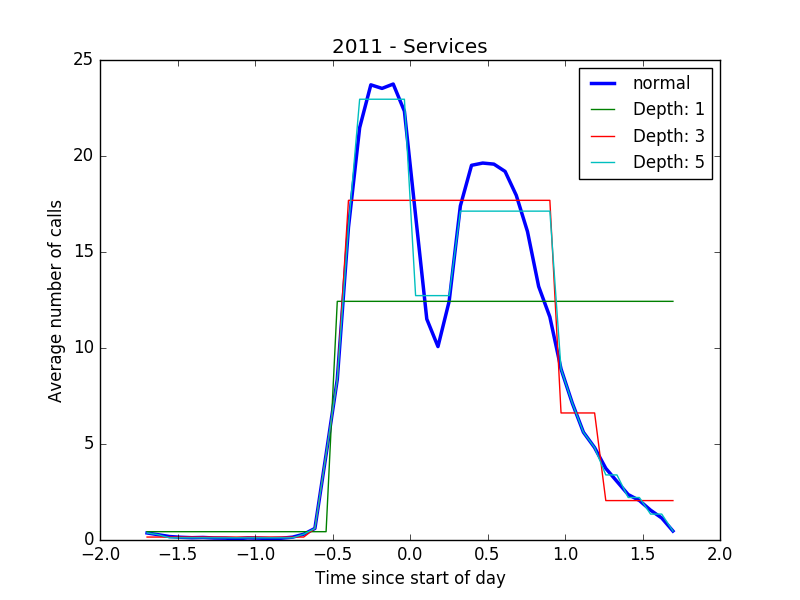
\includegraphics[width=\textwidth]{graphics/1-TreeRegression.png}
      \caption{Performance of several trees with regards to their depth}
      \label{treePerf}
    \end{minipage}
    \hfill
    \begin{minipage}{0.48\textwidth}
      \centering
      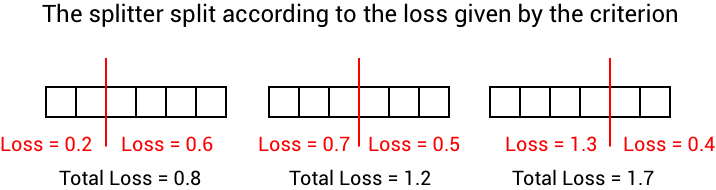
\includegraphics[width=\textwidth]{graphics/splitterpng.png}
      \caption{Visualisation of different splits}
      \label{splitting}
    \end{minipage}
  \end{figure}
  By default, the available criterions in {\tt scikit-learn} are Mean Square Estimator and Mean Absolute Estimator. However, in this assignment, the loss function used to compute the total error at the end is known as linEx, and is defined by :
  \begin{equation}
    \text{linEx}(y,\hat{y}) = \exp \left( \alpha (y-\hat{y})\right) - \alpha (y-\hat{y}) -1
  \end{equation}
  where $y$ is the value of a given data sample $x$, and $\hat{y}$ is its predicted value.

  Since this function will be used to judge the final results of the regression, it seemed interesting to us to implement this function as a possible criterion of the {\tt scikit-learn}. This tweak required to fork from the {\tt scikit-learn} repository and to modify the source files, written in a {\tt C++}-based language called cython in order to add an "lineEx" criterion option for the decision tree regressor.

  However, comptutation of the loss functin over the whole data set required precision up to 60 digits over the values, which is not achievable by using {\tt double} (their precision is limited by their 64bit size). We then chose to use the MSE as the loss function to split the tree, but then using the linEx function to compute the node value. This method seemed to be an acceptable compromise between precision and computation cost (using 60-digit precision integers would multiply by four the computational time and memory cost). Figure \ref{tree_example} shows an example of a tree built using this methodology, as displayed with the {\tt export\_graphviz} function.
  \begin{figure}
    \centering
    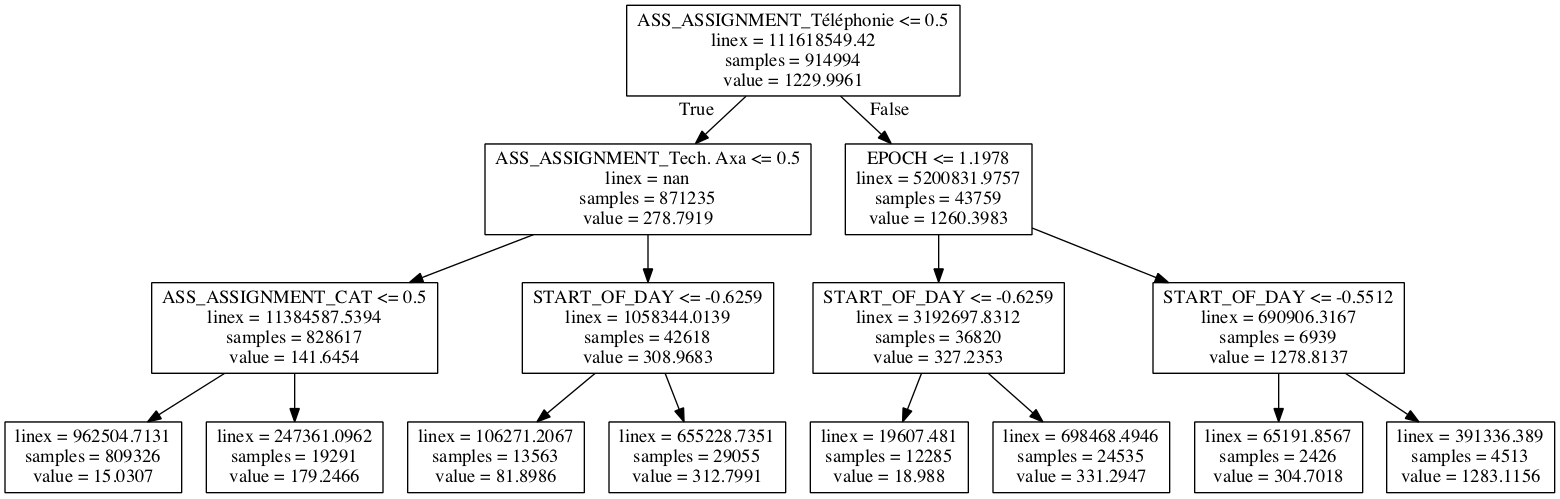
\includegraphics[width=0.8\textwidth]{graphics/tree.png}
    \caption{An example of tree built with the linEx criterion}
      \label{tree_example}
  \end{figure}

  \subsection{Use of decision trees}

  We then used decision trees in two different regression methods : \emph{bagging} and \emph{random forests}.

  The first algorithm of this type we tried was \emph{random forests}. In this leaner, several decision trees are build over several random samples of data and features from the training date. For every test data point, its predicted value is then the mean of the values returned by each tree. We see in figure \ref{forest} that these learners perform slightliy better than a single tree. However, the computational cost is much higher, making them less efficient for practical use.

  \begin{figure}
    \begin{minipage}{0.48\linewidth}
      \centering
      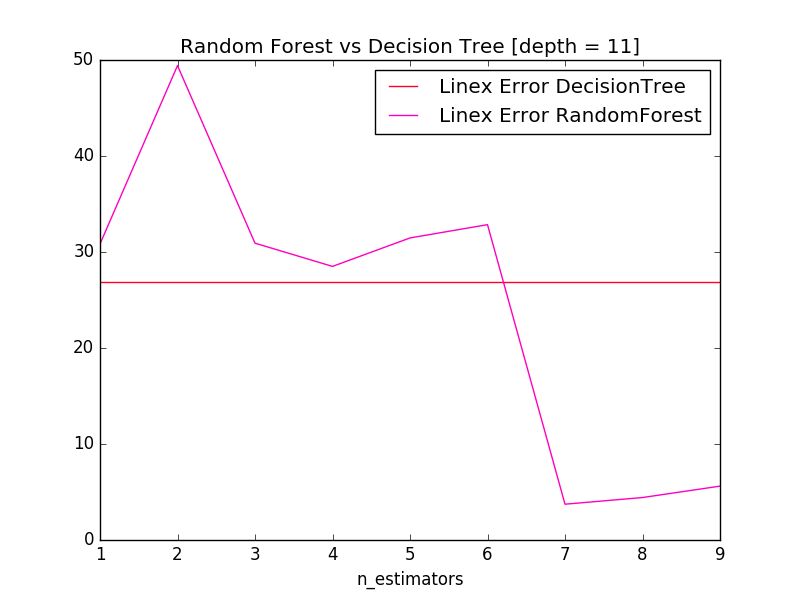
\includegraphics[width=\textwidth]{graphics/forest.png}
      \caption{Perforomance of random forests for various sizes}
      \label{forest}
    \end{minipage}
    \hfill
    \begin{minipage}{0.48\linewidth}
      \centering
      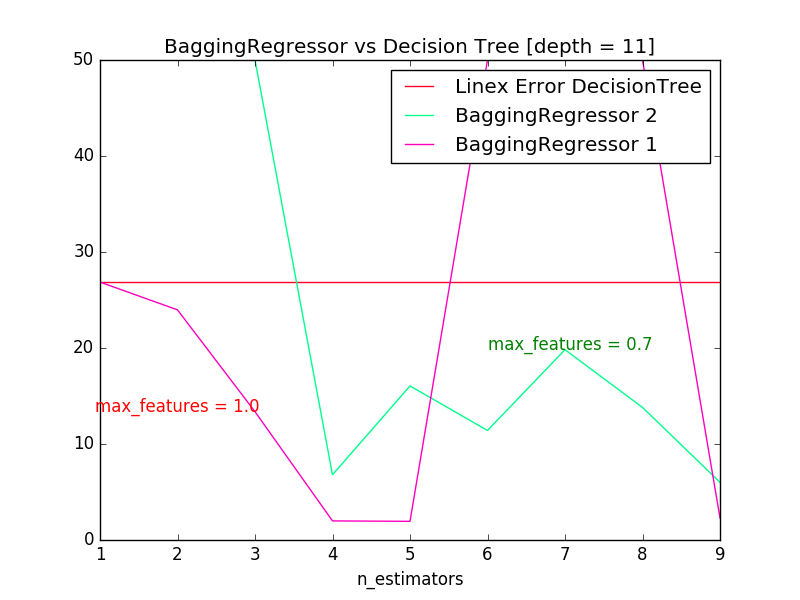
\includegraphics[width=\textwidth]{graphics/Bagging.png}
      \caption{Performance of Bagging algorithms based on decision trees}
      \label{bagging}
    \end{minipage}
  \end{figure}

  A second approach was to use the built-in \emph{bagging} regressor, implemented with the {\tt BaggingRegressor} class in {\tt scikit-learn}. This regressor used our decision tree with linEx criterion as its weak regressor. Its performance is shown in Figure \ref{bagging} and compared to the score of a single decision tree. We can observe that the gain is not overwhelming, and a phenomenon of overfitting seems to appear when taking into account every feature.

  However, due to the high computational cost of such methods, we were not able to further test them, in particular use ensembles of hundreds of decision trees. This limitied the impact of these learners, as they are supposed to scale with the number of weak learners wrapped within them.

  \subsection{Tracks for improvement}

  Using time series analysis on the training data, we observed that our data is mostly time-independant, which means that its statiscal features such as mean, variance and covariance do not evolve much throughout time. Such properties could be used to tune our regression models and get finer results, but due to a lack of time, wh chose to focus on the work thereabove explained.

  \begin{figure}
    \centering
    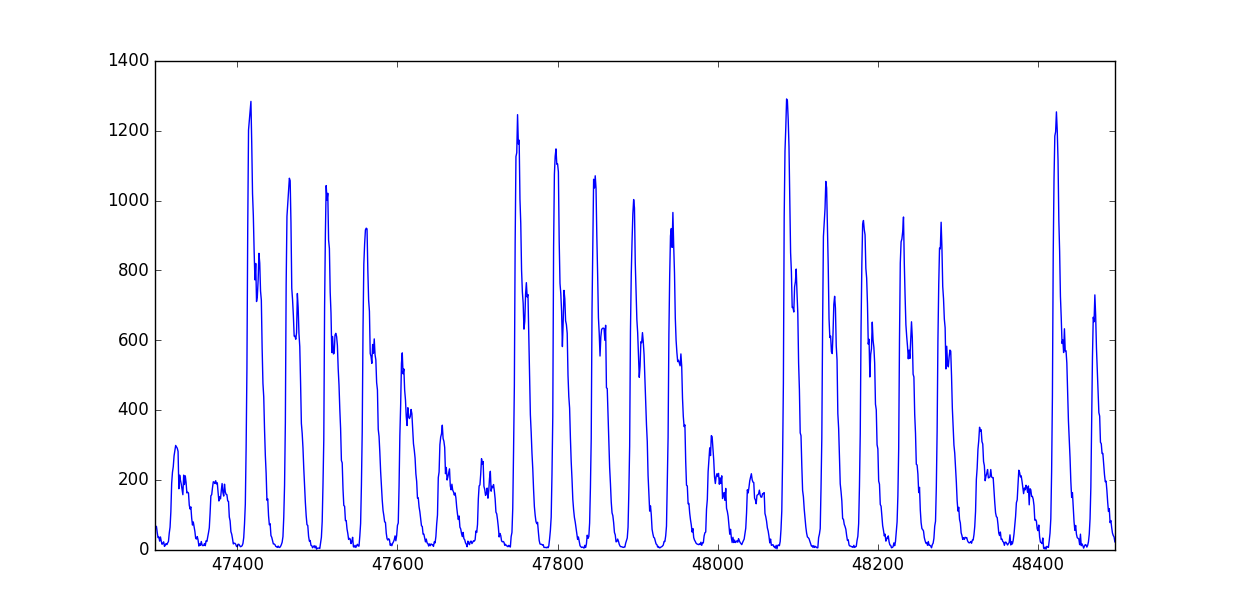
\includegraphics[width=0.8\textwidth]{graphics/3-Time_series.png}
    \caption{Evolution of the data with regards to the time}
    \label{time_series}
  \end{figure}

\part{Conclusion}

  For our team, the best results for this task were achieved by performing random forests regression after tweaking the decision trees provided by {\tt scikit-learn} to take into account the linEx loss function as a criterion.

  Our hardware limitations prevented us from performing further tests with higher forest sizes, but significant improvements are to be expected, given the  performance gap between a single tree and a 10 tree strong forest.

  Others particularities of our dataset, such as its relative time-independance, have been remarked but are not yet used and could lead to further progress.

%   \subsection*{The Linex loss function}
%
%
% \vspace{1 cm}
% \label{norms}
% We have the loss function defined by:
%     $$loss = \sum_{i=1}^{n} (e^{\alpha (y_i-y_{pred})} - \alpha  (y_i-y_{pred}) - 1)$$
%
%
% Its \textbf{derivative} defined by:
%     $$ \frac{\partial loss}{\partial y_{pred}} = \sum_{i=1}^{n} (-\alpha e^{\alpha (y_i-y_{pred})} + \alpha)$$
%     $$ \frac{\partial loss}{\partial y_{pred}} = -\alpha e^{-\alpha y_{pred}} \sum_{i=1}^{n} ( e^{\alpha y_i} ) + n\alpha$$
%
%
%
%
% Looking for the \textbf{minimum}, we have:
%     $$ \frac{\partial loss}{\partial y_{pred}} = 0 \implies
%     e^{\alpha y_{pred}} = \frac{\sum_{i=1}^{n} (e^{\alpha y_i})}{n}$$
%     $$ y_{pred} = \frac{1}{\alpha} \log(\frac{\sum_{i=1}^{n} (e^{\alpha y_i})}{n})$$
%
%
%
%
% Replacing this value in the loss, we obtained the \textbf{minimum loss}, ie. the minimum impurity of the data.
%     $$loss = n\log(\frac{\sum_{i=1}^{n} (e^{\alpha y_i})}{n}) - \sum_{i=1}^{n} \alpha y_i$$
%
%
%
%
% And we can verify, using the Jensen inequality that:
%     $$loss >= 0$$



\end{document}
